\documentclass{beamer}
\usepackage{amsmath}
\usepackage[english]{babel} %set language; note: after changing this, you need to delete all auxiliary files to recompile
\usepackage[utf8]{inputenc} %define file encoding; latin1 is the other often used option
\usepackage{csquotes} % provides context sensitive quotation facilities
\usepackage{graphicx} %allows for inserting figures
\usepackage{booktabs} % for table formatting without vertical lines
\usepackage{textcomp} % allow for example using the Euro sign with \texteuro
\usepackage{stackengine}
\usepackage{wasysym}
\usepackage{tikzsymbols}
\usepackage{textcomp}
\newcommand{\bubblethis}[2]{
        \tikz[remember picture,baseline]{\node[anchor=base,inner sep=0,outer sep=0]%
        (#1) {\underline{#1}};\node[overlay,cloud callout,callout relative pointer={(0.2cm,-0.7cm)},%
        aspect=2.5,fill=yellow!90] at ($(#1.north)+(-0.5cm,1.6cm)$) {#2};}%
    }%
\tikzset{face/.style={shape=circle,minimum size=4ex,shading=radial,outer sep=0pt,
        inner color=white!50!yellow,outer color= yellow!70!orange}}
%% Some commands to make the code easier
\newcommand{\emoticon}[1][]{%
  \node[face,#1] (emoticon) {};
  %% The eyes are fixed.
  \draw[fill=white] (-1ex,0ex) ..controls (-0.5ex,0.2ex)and(0.5ex,0.2ex)..
        (1ex,0.0ex) ..controls ( 1.5ex,1.5ex)and( 0.2ex,1.7ex)..
        (0ex,0.4ex) ..controls (-0.2ex,1.7ex)and(-1.5ex,1.5ex)..
        (-1ex,0ex)--cycle;}
\newcommand{\pupils}{
  %% standard pupils
  \fill[shift={(0.5ex,0.5ex)},rotate=80] 
       (0,0) ellipse (0.3ex and 0.15ex);
  \fill[shift={(-0.5ex,0.5ex)},rotate=100] 
       (0,0) ellipse (0.3ex and 0.15ex);}

\newcommand{\emoticonname}[1]{
  \node[below=1ex of emoticon,font=\footnotesize,
        minimum width=4cm]{#1};}
\usepackage{scalerel}
\usetikzlibrary{positioning}
\usepackage{xcolor,amssymb}
\newcommand\dangersignb[1][2ex]{%
  \scaleto{\stackengine{0.3pt}{\scalebox{1.1}[.9]{%
  \color{red}$\blacktriangle$}}{\tiny\bfseries !}{O}{c}{F}{F}{L}}{#1}%
}
\newcommand\dangersignw[1][2ex]{%
  \scaleto{\stackengine{0.3pt}{\scalebox{1.1}[.9]{%
  \color{red}$\blacktriangle$}}{\color{white}\tiny\bfseries !}{O}{c}{F}{F}{L}}{#1}%
}
\usepackage{fontawesome} % Social Icons
\usepackage{epstopdf} % allow embedding eps-figures
\usepackage{tikz} % allows drawing figures
\usepackage{amsmath,amssymb,amsthm} %advanced math facilities
\usepackage{lmodern} %uses font that support italic and bold at the same time
\usepackage{tikz}

\usepackage{tcolorbox}

\usefonttheme[onlymath]{serif} %set math font to serif ones

\definecolor{beamerblue}{rgb}{0.2,0.2,0.7} %define beamerblue color for later use

%%% defines highlight command to set text blue
\newcommand{\highlight}[1]{{\color{blue}{#1}}}


%%%%%%% commands defining backup slides so that frame numbering is correct

\newcommand{\backupbegin}{
   \newcounter{framenumberappendix}
   \setcounter{framenumberappendix}{\value{framenumber}}
}
\newcommand{\backupend}{
   \addtocounter{framenumberappendix}{-\value{framenumber}}
   \addtocounter{framenumber}{\value{framenumberappendix}}
}

%%%% end of defining backup slides

%Specify figure caption, see also http://tex.stackexchange.com/questions/155738/caption-package-not-working-with-beamer
\setbeamertemplate{caption}{\insertcaption} %redefines caption to remove label "Figure".
%\setbeamerfont{caption}{size=\scriptsize,shape=\itshape,series=\bfseries} %sets figure  caption bold and italic and makes it smaller


\usetheme{Boadilla}

% --------------------
% Overall information
% --------------------
\title[Economía I]{Economía I \vspace{4mm}
\\ Magistral 24: Mercado de dinero}
\date{}
\author[Riottini]{Riottini Franco}
\vspace{0.4cm}
\institute[]{Universidad de San Andrés} 


\begin{document}

\begin{frame}
\titlepage
\centering

\includegraphics[scale=0.2]{../Figures/logoUDESA.jpg} 
\end{frame}

\begin{frame}{Las funciones del dinero}
    \begin{itemize}
        \item \textbf{Medio de cambio}: el dinero es utilizado como un mecanismo para realizar transacciones $\rightarrow$ fundamental la confianza
        \item \textbf{Unidad de cuenta}: el dinero es también una medida que sirve para definir precios así como para registrar activos y deudas $\rightarrow$ corroido por la inflación
        \item \textbf{Depósito de valor}: el dinero permite transferir poder adquisitivo del presente al futuro $\rightarrow$ corroido por la inflación
   \end{itemize}
\end{frame}

\begin{frame}{Tipos de dinero}
    \begin{itemize}
        \item Durante la mayor parte de la historia de la humanidad se utilizó dinero mercancía (commodity money)
            \begin{itemize}
                \item Mercancías con valor intrínseco que se usaban para comerciar: Oro, plata, sal, cigarrillos, etc.
            \end{itemize}
        \item Hoy en día, casi todo el dinero es fiduciario (fiat money)               
        \begin{itemize}
            \item Sin valor intrínseco, pero que se utiliza porque el gobierno lo hace de curso legal: Pesos, euros, dólares, bonos provinciales (cuasimonedas), etc.
            \item Ahora es casi natural, pero tomó mucho tiempo: Problemas de confianza, falsificación, funcionamiento, etc.
        \end{itemize}
    \end{itemize}
\end{frame}

\begin{frame}{Commodity money}
            \begin{figure} [H]   
  \centering
  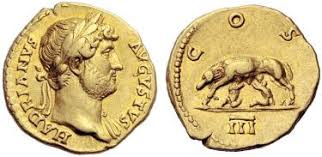
\includegraphics[width=.8\textwidth]{../Figures/C32.1.jpg}
      \caption{Monedas carcomidas}
\end{figure}
\end{frame}

\begin{frame}{Dinero Papel}
    \begin{itemize}
        \item Comienza a usarse en China en el Siglo VII
        \item Antes de los bancos centrales los emitían los bancos 
        
\begin{figure} [H]   
  \centering
  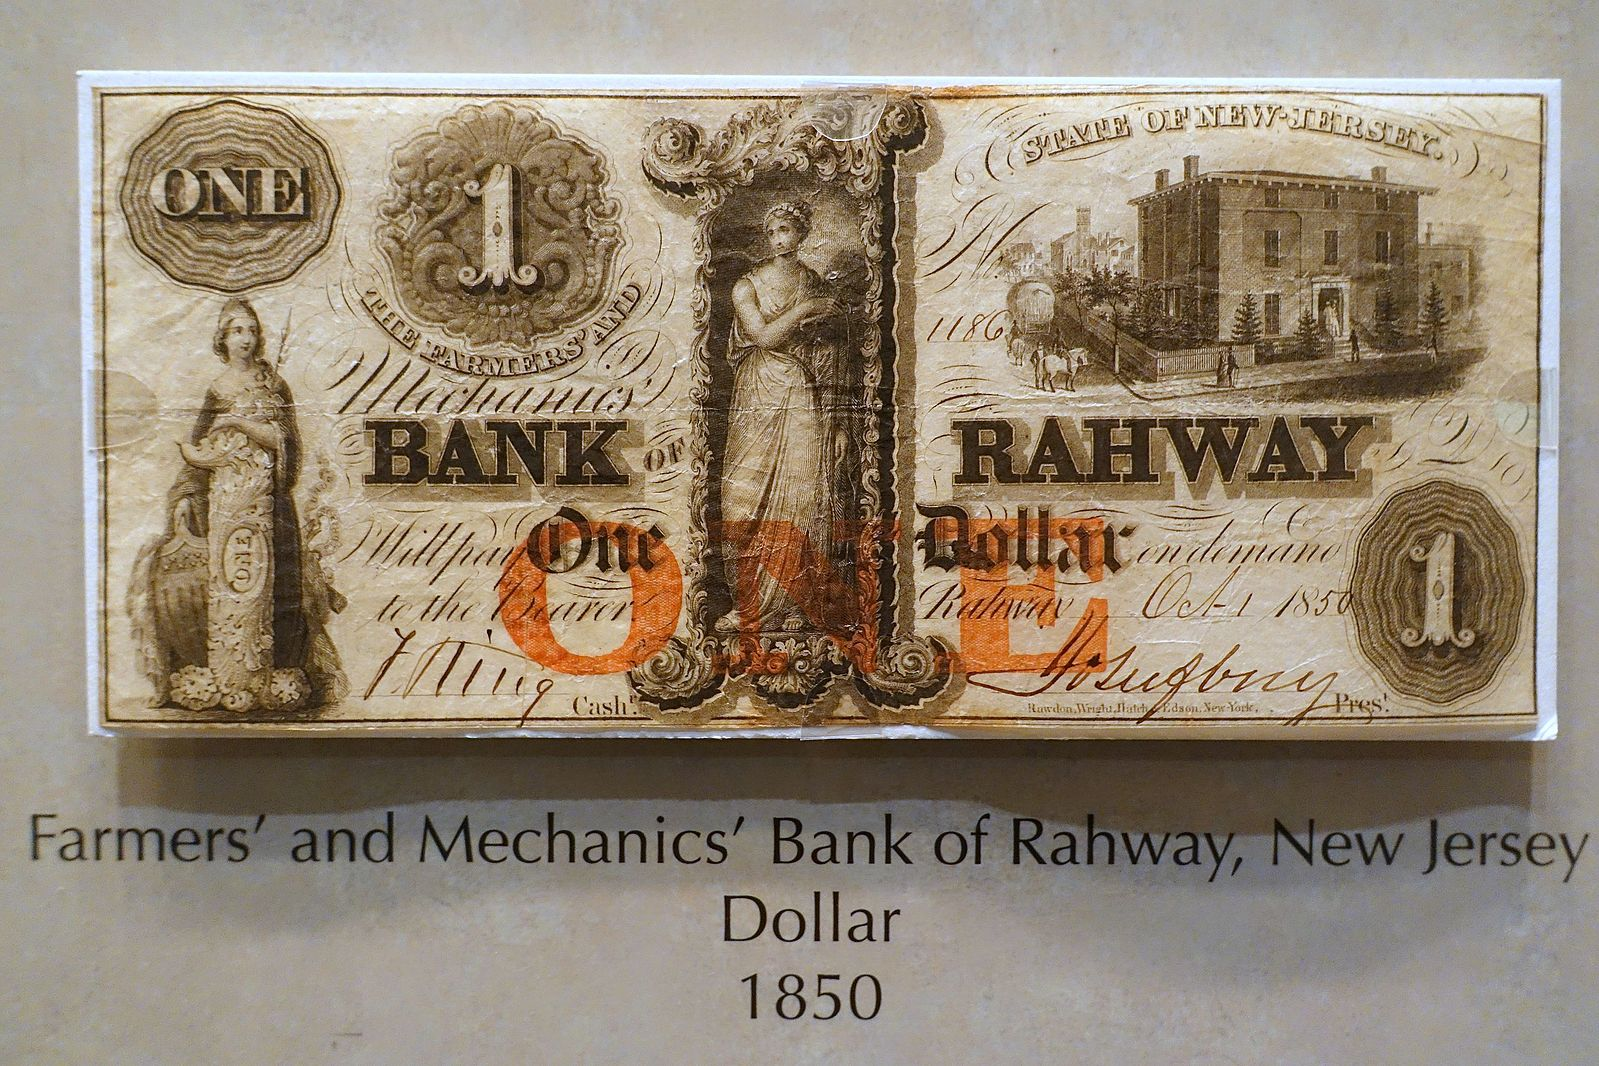
\includegraphics[width=.35\textwidth]{../Figures/C32.2.jpg}
      \caption{Dollar de Bank of Rahway, New Jersey, 1850. Via Wikimedia Commons}
  \label{fig:C32.2}
\end{figure}

\begin{figure} [H]   
  \centering
  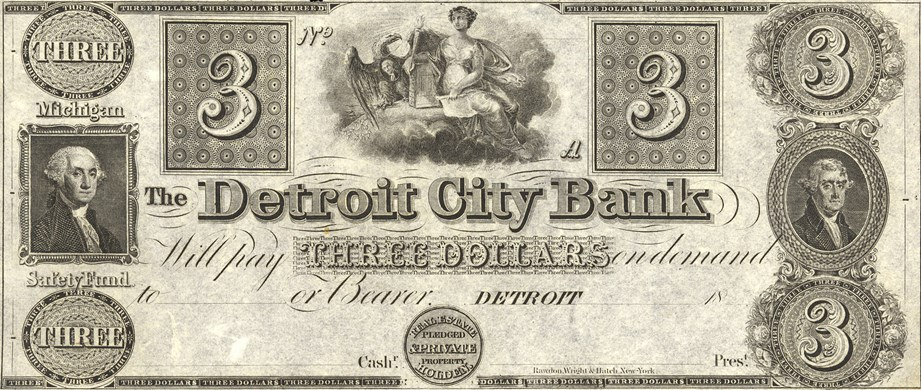
\includegraphics[width=.35\textwidth]{../Figures/C32.3.jpeg}
      \caption{Detroit City Bank \$3 Note}
  \label{fig:C32.3}
\end{figure}
\end{itemize}
\end{frame}
        
\begin{frame}{El dinero}
        \begin{figure} [H]   
  \centering
  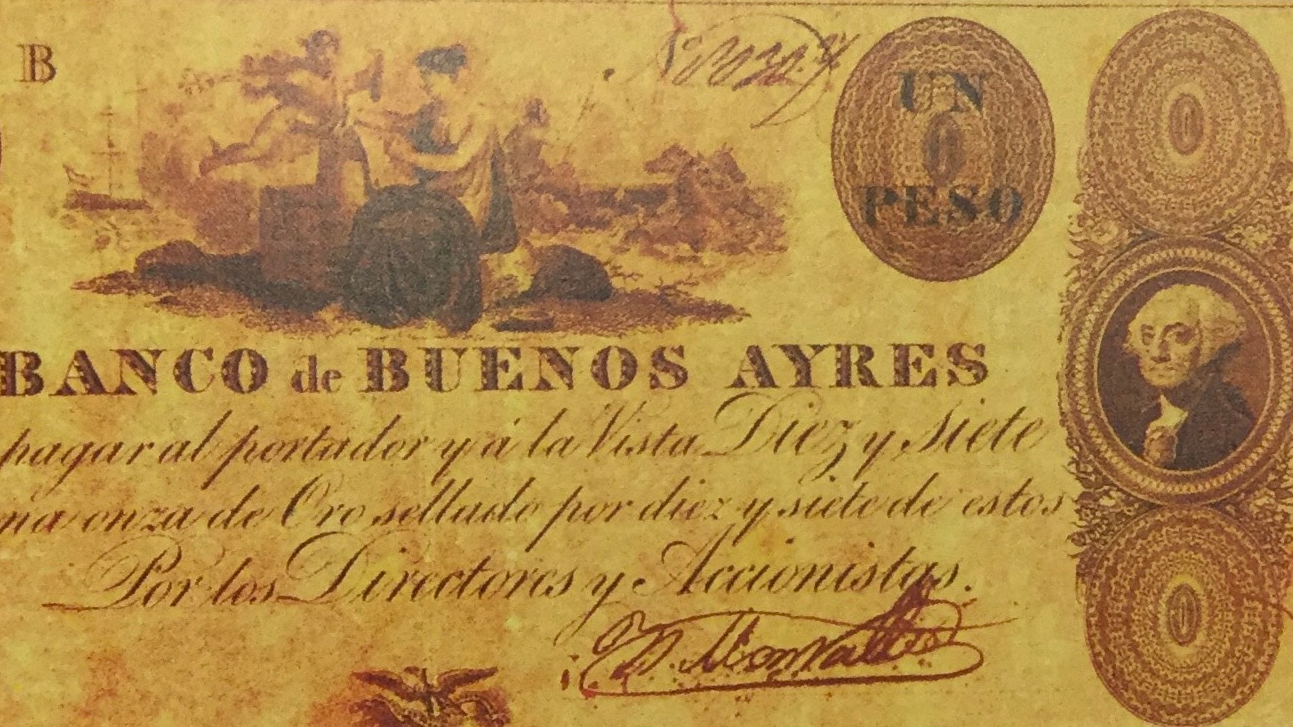
\includegraphics[width=.35\textwidth]{../Figures/C32.4.jpg}
      \caption{Billetes emitidos por el Banco Provincia de Buenos Aires}
  \label{fig:C32.4}
\end{figure}

\begin{figure} [H]   
\centering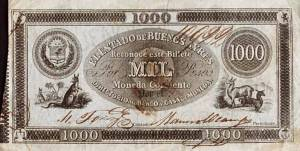
\includegraphics[width=.35\textwidth]{../Figures/C32.5.jpg}
\caption{Billetes emitidos por el Banco Provincia de Buenos Aires}
\end{figure}
       \begin{itemize}
           \item  Luego lo monopolizaron los bancos centrales
    \item Y hoy volvemos a la multiplicidad de monedas 
       \end{itemize}     
        \end{frame}


\begin{frame}{La demanda de dinero}
    \begin{itemize}
        \item La demanda de dinero es lo que la gente demanda de dinero, es cuánto dinero desea tener la sociedad
        \item Se explica por dos motivos principalmente: por motivo \textbf{transaccional} y por motivo \textbf{especulativo}
        \begin{itemize}
        \item Por transacciones $\Rightarrow P*Y \Rightarrow$ a mayores precios o mayor nivel de actividad aumenta la demanda de dinero por transacciones
        \item Costo de oportunidad $\Rightarrow i \Rightarrow $ la demanda de dinero depende negativamente de la tasa de interés que es el costo de oportunidad del dinero
    \end{itemize}
    \item La llegada de las tarjetas de crédito, el dinero bancario y la agilidad de transferir dinero de activos líquidos a dinero, entre otros, son elementos que han ido cambiando drásticamente la demanda de dinero en el tiempo
    \end{itemize}
\end{frame}

\begin{frame}{La oferta de dinero}
    \begin{itemize}
       \item Oferta primaria. Determinada por el Banco Central que incluye en la base monetaria.
       \item Oferta secundaria. Dinero creado por los bancos comerciales al otorgar créditos a partir de depósitos.
       \end{itemize}
\end{frame}

\begin{frame}
\frametitle{¿Qué es el Banco Central?}
\begin{itemize}
    \item Un banco particular
        \begin{itemize}
            \item Es generalmente propiedad del gobierno.
            \item Actúa como banquero de los bancos comerciales: Que tienen `reservas' en el Banco Central.
            \item Es prestamista de ultima instancia.
            \item Es el único que puede crear moneda de curso legal.
        \end{itemize}
    \item Dinero en el sentido amplio
        \begin{itemize}
            \item Base monetaria (base money) o M0: Billetes y monedas, más cuentas depositadas en el Banco Central (encajes).
            \item Depósitos (bank money): Dinero creado por los bancos comerciales al extender crédito.
        \end{itemize}
\end{itemize}
\end{frame}

\begin{frame}{El balance del Banco Central}
        \begin{figure} [H] 
            \centering
            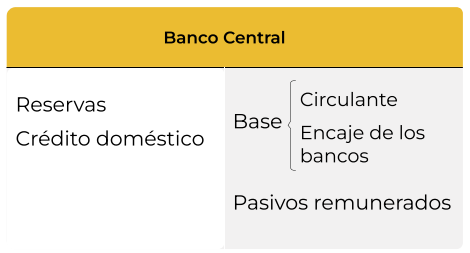
\includegraphics[width=6.5cm]{../Figures/C37.8.png}
        \end{figure}
        \begin{figure} [H] 
            \centering
            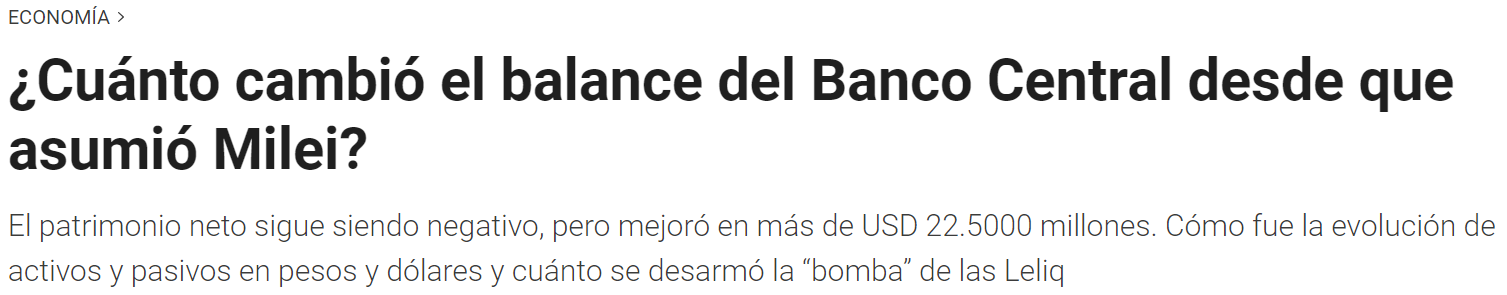
\includegraphics[width=8.5cm]{../Figures/Mejora_Balance_Central.png}
        \end{figure}
\end{frame}

\begin{frame}{¿Qué más hace el Banco Central?}
    \begin{itemize}
        \item Crea y regula la cantidad de dinero en la economía
        \item Regula la actividad bancaria
        \item Es prestamista de última instancia
        \item Maneja la política cambiaria 
    \end{itemize}
\end{frame}

\begin{frame}
\frametitle{¿Qué son los bancos?}
\begin{itemize}
    \item Son intermediarios financieros
    \item Instituciones que reciben fondos de personas y empresas, y los utilizan para comprar bonos o acciones, o para hacer préstamos a otros agentes
    \begin{itemize}
        \item Los bancos piden prestado a los hogares (depósitos), otros bancos, y el banco central \\
        \item El interés que pagan por los depósitos (tasa de interés pasiva) es menor que el que cobran en préstamos (tasa de interés activa, lending rate), y así obtienen beneficios:
        \[ \text{Spread} = \text{Interés activo} - \text{Interés pasivo} \]
    \end{itemize}
\end{itemize}
\end{frame}

\begin{frame}{Riesgos que tienen que manejar los bancos}
    \begin{itemize}
        \item \textbf{Riesgo de credito o default}: Riesgo de que los créditos del banco no sean repagados
        \item \textbf{Riesgo de madurez}: Riesgo de que los activos y pasivos del banco no tengan la misma duración
        \item \textbf{Riesgo de liquidez}: Riesgo de que el activo no se pueda transformar en efectivo (liquidar) sin generar una pérdida financiera
    \end{itemize}
    Estos riesgos pueden hacer que los depositantes no tomen las decisiones más correctas, lo que puede generar riesgos sistémicos. El banco central ayuda a mitigar este riesgo (principalmente de \textit{corridas}) obligando a los bancos a guardar un porcentaje de los depósitos (encajes). 
\end{frame}


\begin{frame}{El multiplicador monetario}
    \begin{itemize}
        \item Los bancos comerciales también crean dinero.
        \item Surge de su posibilidad de entregar créditos.
        \item La llamamos creación secundaria de dinero.
        \item Es afectado por la tasa de encajes y por la preferencia por la liquidez.
        \item Los encajes se usan para regular la cantidad de dinero
    \end{itemize}
\end{frame}

\begin{frame}{El multiplicador monetario}
    \begin{itemize}
        \item Ejemplo:  circulante = 100  y  encajes = 10\%:

        \begin{center}
            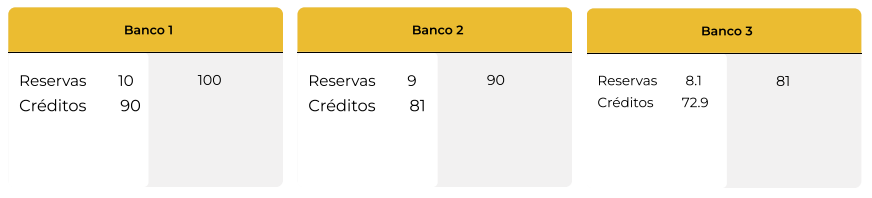
\includegraphics[width=9cm]{../Figures/C37.15.png}
    
            \[M1 = \text{circulante} + \text{depósitos} = 100 + 90 + 81 + 72.9 + ..... = 1000 \]
        \end{center}
        \item Otro ejemplo:  circulante = 100  y  encajes = 20\%:
            
        \begin{center}
            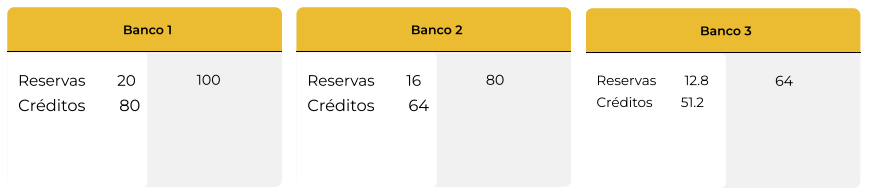
\includegraphics[width=9cm]{../Figures/C37.16.png}
    
            \[M1 = \text{circulante} + \text{depósitos} = 100 + 80 + 64 + 51.2 + ..... = 500 \]
        \end{center}
    \end{itemize}
\end{frame}


\begin{frame}{Los agregados monetarios}
    \begin{itemize}
        \item M0 = Base monetaria = Circulante + Encajes bancarios
        \item M1 = Circulante + Depósitos en cuenta corriente
        \item M2 = M1 + Caja de Ahorro
        \item M3 = M2 + Plazo Fijo
        \item M? = M3 + saldos de tarjetas?, programa de millajes? 
        \item etc.
    \end{itemize}
\end{frame}

\end{document}